\documentclass{report}
\usepackage[margin=1in, paperwidth=8.5in, paperheight=11in]{geometry}
%Math packages%
\usepackage{amsmath}
\usepackage{amssymb}
\usepackage{amsthm}
%Spacing%
\usepackage{setspace}
\onehalfspacing
%Lecture number%
\newcommand{\lectureNum}{15}
%Variables - Date and Course%
\newcommand{\curDate}{February 6, 2017}
\newcommand{\course}{MATH 239}
\newcommand{\instructor}{Luke Postle}
%Defining the example tag%
%\theoremstyle{definition}%
\newtheorem{ex}{Example}[section]
%Setting counter given the lecture number%
\setcounter{chapter}{\lectureNum{}}
%Package for drawing graphs%
\usepackage{tikz}
\usepackage{verbatim}
\usetikzlibrary{arrows}

\begin{document}
%Note title%
\begin{center}
\begin{Large}
\textsc{\course{} | Lecture \lectureNum{}}
\end{Large}
\end{center} 
\noindent \textit{Bartosz Antczak} \hfill
\textit{Instructor: \instructor{}} \hfill
\textit{\curDate{}}
\rule{\textwidth}{0.4pt}

% Actual Notes%
\subsubsection{Review of Last Lecture}
A \textbf{platonic solid} is a plane graph where all vertices have the same degree $d$ and all faces have the same degree $d^*$. A \textbf{theorem} we discussed was
\begin{center}
\textit{There are exactly five platonic solids: the tetrahedron, cube, octahedron, icosahedron, dodecahedron}
\end{center}
(A visual of these platonic solids was shown last lecture). Additionally, we covered a \textbf{lemma}:
\begin{center}
\textit{If G is a platonic solid, then $(d, d^*) \in \{(3,3),(3,4),(4,3),(3,5),(5,3)\}$}
\end{center}
Now recall: $$2E = d^*F = dV \qquad \text{(By handshaking + handshaking for faces)}$$
By Euler's formula:
\begin{align*}
&\implies V - E + F = 2 \\
&\implies \frac{2E}{d} - E + \frac{2E}{d^*} = 2 \\
&\implies E = \frac{2dd^*}{2(d+d^*)-dd^*} && (\text{Solving for }E)
\end{align*}
\section{Proof of there being only 5 Platonic Solids}
To prove that there are only five platonic solids, we must show that the only solid with a particular $(d, d^*)$ pairing, then it's the \textit{only} one in our list. We consider 5 cases (we'll prove only the first two):
\subsection{Lemma 1}
\begin{center}
\textit{If G is a platonic solid with $d = d^* = 3$, then G is the tetrahedron}
\end{center}
\subsubsection{Proof of Lemma 1}
By calculation, $V = 4$, and $E=6$. But then $G$ is $K_4$, which only has one planar embedding (and $F=4$) (i.e., $G$ is the tetrahedron).
\subsection{Lemma 2}
\begin{center}
\textit{If G is a platonic solid with $d = 3, d^* = 4$, then G is the cube}
\end{center}
\subsubsection{Proof of Lemma 2}
By calculation, given our $(d, d^*)$, $V = 8$, $E = 12$, and $F = 6$. Let $G$ be such a solid. Let $f$ be a face of $G$. Note that $f$ has degree 4 and so is a 4-cycle $C = v_1v_2v_3v_4$.
We claim that $v_1$ is not adjacent to $v_3$. Suppose not, then the other face $f^\prime$ containing $v_1v_4$ must also contain $v_1v_3$, $v_4v_3$, and $v_4w$ (twice) where $w$ is the other neighbour of $v_4$. But then $\mathrm{deg}(f^\prime) = 5$, a contradiction. This proves the claim that $v_1$ is not adjacent to $v_3$. By symmetry, $v_2$ is not adjacent to $v_4$.\\
Let $u_i$ be the other neighbour of $v_i$. Now I claim that all $u_i$ are distinct. To prove this, suppose not. There are 2 cases up to symmetry:
\begin{itemize}
\item \textbf{Case 1:} $u_1 = u_2$. But then the other face containing $v_1v_2$ is either a triangle or has degree greater than or equal to 5. a contradiction.
\item \textbf{Case 2:} $u_1=u_3$. But then, $u_2$ must be adjacent to $u_1=u_3$ for the face containing $v_1v_2$ to be a 4-cycle. But then $u_2$ has degree 2, a contradiction.
\end{itemize}
But now $u_iu_{i+1(\mathrm{mod} 4)}$ is an edge since the face containing $v_iv_{i+1(\mathrm{mod} 4)}$ is a 4-cycle. But then $G$ is the cube, as desired.
\section{Let's Return to the Big Question}
\textbf{When is a graph $G$ planar?}\\
We begin by analysing if this decision problem is in either $P$, $NP$, or co$-NP$. Observe that we can just check an embedding in polynomial time, which means that it's true for $NP$.\\
But what about co$-NP$? It's not obvious since there are exponentially many embeddings. It turns out that the answer is in fact \textit{yes}, which will be proven by corollary 2 at the end of this lecture.\\
Recall:
\begin{center}
\textit{If $G$ is planar, then G does not have a non-planar subgraph (e.g., $K_5$ or $K_{3,3}$)}
\end{center}
We'll begin with a definition:
\subsubsection{Definition | Subdivide}
If $G$ is a graph and $e = uv \in E(G)$, then to \textbf{subdivide} $e$ is to delete it and add a new vertex $w$ adjacent to both $u$ and $v$:
\begin{center}
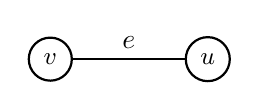
\begin{tikzpicture}[-,auto,node distance=2cm,
                    thick,main node/.style={circle,draw,font=\sffamily\small}]

  \node[main node] (1) {$v$};
  \node[main node] (2) [right of=1] {$u$};
  
  \path[every node/.style={font=\sffamily}]
    (1) edge node [above] {$e$} (2);
\end{tikzpicture}
$\qquad\qquad \implies \qquad\qquad$
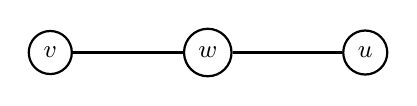
\begin{tikzpicture}[-,auto,node distance=2cm,
                    thick,main node/.style={circle,draw,font=\sffamily\small}]

  \node[main node] (1) {$v$};
  \node[main node] (2) [right of=1] {$w$};
  \node[main node] (3) [right of=2] {$u$};
  
  \path[every node/.style={font=\sffamily}]
    (1) edge (2)
    (2) edge (3);
\end{tikzpicture}
\end{center}
\subsubsection{Definition | Subdivisions (Not the Rush song)}
A \textbf{subdivision} of a graph $H$ (also called an $H-$subdivision) is a graph obtained from $H$ by subdividing edges (those edges had to be cool or be cast out).\\
We will use this definition determine when a graph is planar using the following lemma:
\subsection{Lemma 3}
Let $H$ be a subdivision of $G$. Then,
\begin{center}
\textit{H is planar $\iff$ G is planar}
\end{center}
\subsubsection{Proof of Lemma 3}
\begin{itemize}
\item \textbf{($\impliedby$):} if $G$ is planar, then just subdivide its planar embedding to get a planar embedding of $H$.
\item \textbf{($\implies$):} if $H$ is planar, then in a planar embedding, replace the paths of degree 2 with the original edges of $G$ to get a planar embedding of $G$ (i.e., `unsubdivide').
\end{itemize}
\subsection{Corollary 1}
\begin{center}
\textit{If G is planar, then G does not contain (as a subgraph) a $K_5-$subdivision or $K_{3,3}-$subdivision}
\end{center}
So not having a $K_5-$subdivision or a $K_{3,3}-$subdivision is a necessary condition to be planar. Surprisingly, it's also a sufficient condition. This leads to Kuratowski's theorem.
\subsection{Kuratowski's Theorem}
\begin{center}
\textit{G is planar $\iff$ G contains no $K_5-$subdivision or $K_{3,3}-$subdivision}
\end{center}
\subsection{Corollary 2}
\begin{center}
\textit{Deciding planarity is in co$-NP$}
\end{center}
\subsubsection{Proof of Corollary 2}
Simply show the $K_5$ or $K_{3,3}-$subdivision.
%END%
\end{document}